%%%%%%%%%%%%%%%%%%%%%%%%%%%%%%%%%%%%%%%%%
% Homework Assignment Article
% LaTeX Template
% Version 1.3.1 (ECL) (08/08/17)
%
% This template has been downloaded from:
% Overleaf
%
% Original author:
% Victor Zimmermann (zimmermann@cl.uni-heidelberg.de)
%
% License:
% CC BY-SA 4.0 (https://creativecommons.org/licenses/by-sa/4.0/)
%
%%%%%%%%%%%%%%%%%%%%%%%%%%%%%%%%%%%%%%%%%

%----------------------------------------------------------------------------------------

\documentclass[a4paper]{article} % Uses article class in A4 format

%----------------------------------------------------------------------------------------
%	FORMATTING
%----------------------------------------------------------------------------------------

\addtolength{\hoffset}{-2.25cm}
\addtolength{\textwidth}{4.5cm}
\addtolength{\voffset}{-3.25cm}
\addtolength{\textheight}{5cm}
\setlength{\parskip}{0pt}
\setlength{\parindent}{0in}

%----------------------------------------------------------------------------------------
%	PACKAGES AND OTHER DOCUMENT CONFIGURATIONS
%----------------------------------------------------------------------------------------

\usepackage{blindtext} % Package to generate dummy text
% \usepackage[style=numeric,sorting=none]{biblatex}
\usepackage{charter} % Use the Charter font
\usepackage[utf8]{inputenc} % Use UTF-8 encoding
\usepackage{microtype} % Slightly tweak font spacing for aesthetics

\usepackage[english]{babel} % Language hyphenation and typographical rules

\usepackage{amsthm, amsmath, amssymb} % Mathematical typesetting
\usepackage{float} % Improved interface for floating objects
\usepackage[final, colorlinks = true, 
            linkcolor = black, 
            citecolor = black]{hyperref} % For hyperlinks in the PDF
\usepackage{graphicx, multicol} % Enhanced support for graphics
\usepackage{xcolor} % Driver-independent color extensions
\usepackage{marvosym, wasysym} % More symbols
\usepackage{rotating} % Rotation tools
\usepackage{censor} % Facilities for controlling restricted text
\usepackage{listings, style/lstlisting} % Environment for non-formatted code, !uses style file!
\usepackage{pseudocode} % Environment for specifying algorithms in a natural way
\usepackage{style/avm} % Environment for f-structures, !uses style file!
\usepackage{booktabs} % Enhances quality of tables
\usepackage{wrapfig}
\usepackage{tikz-qtree} % Easy tree drawing tool
\tikzset{every tree node/.style={align=center,anchor=north},
         level distance=2cm} % Configuration for q-trees
\usepackage{style/btree} % Configuration for b-trees and b+-trees, !uses style file!

% \usepackage[backend=biber,style=numeric,
            % sorting=nyt]{biblatex} % Complete reimplementation of bibliographic facilities
% \addbibresource{ecl.bib}
\usepackage{csquotes} % Context sensitive quotation facilities

\usepackage[yyyymmdd]{datetime} % Uses YEAR-MONTH-DAY format for dates
\renewcommand{\dateseparator}{-} % Sets dateseparator to '-'

\usepackage{fancyhdr} % Headers and footers
\pagestyle{fancy} % All pages have headers and footers
\fancyhead{}\renewcommand{\headrulewidth}{0pt} % Blank out the default header
\fancyfoot[L]{School of Computing, Macquarie University} % Custom footer text
\fancyfoot[C]{} % Custom footer text
\fancyfoot[R]{\thepage} % Custom footer text

\usepackage{comment}
\newcommand{\note}[1]{\marginpar{\scriptsize \textcolor{red}{#1}}} % Enables comments in red on margin

%----------------------------------------------------------------------------------------

\begin{document}

%----------------------------------------------------------------------------------------
%	TITLE SECTION
%----------------------------------------------------------------------------------------

\title{COMP3100 project report} % Article title
\fancyhead[C]{}
\hrule \medskip % Upper rule
\begin{minipage}{1\textwidth} % Center of title section
\centering 
\large % Title text size
Project report: Stage 1\\ % Assignment title and number
COMP3100 Distributed Systems, S2, 2022\\
\normalsize % Subtitle text size
SID: 45339201, Name: Victor Chan
%%%%\\ % Assignment subtitle
\end{minipage}
\medskip\hrule % Lower rule
\bigskip

%----------------------------------------------------------------------------------------
%	ARTICLE CONTENTS
%----------------------------------------------------------------------------------------
\section{Introduction}
For this Distributed Systems Project, the desired outcome is to create a fully functional Client Server Simulator using Oracle's Virtual-Box \cite{VirtualBox} running on the Ubuntu \cite{Ubuntu} System. The goals involving ds-sims will be outlined below, these goals are reflected in Stage 1 of the COMP3100 Project. In addition, all aspects of this project can be accessed via Github\cite{github}.
\bigskip

In this report, the aim to create a client-side simulator using a job dispatcher which will connect to the server-side simulator, enabling it to receive jobs and sends all jobs to the largest server type. This assignment of jobs will be performed using Largest-Round-Robin (LRR), scheduling largest jobs first based on the number of cores. If there are more than one job with the same amount of cores detected, whichever job was detected first, would be used.
\bigskip

The report will be formatted in this following order:
\bigskip

The rest of this report is organised as follows. Section~\ref{sec:section2} to Section~\ref{sec:section4} gives an overview of:
\begin{itemize}
  \item \textbf{Section 2}: \underline{System Overview}: Depicting the interaction between the server-side and client-side system, outlining the process on how the jobs are to be ran.
  \item \textbf{Section 3}: \underline{Design}: Exploring the client-side simulator, additionally the functionalities and constraints within the project.
  \item \textbf{Section 4}: \underline{Implementation}: Explore how the software libraries, data structures, software and strategies that are applied and implemented to the client-side simulator.
\end{itemize}

\section{System Overview}
\label{sec:section2}
The functionality of the ds-sim displays the process on how the server-side simulator is utilised to dispatch jobs.
\bigskip

Firstly, the server must already be running before the client can connect, the sockets of the client will be running on the localhost (127.0.0.1) and port 50000. Once this connection is made, the client will initiate its communication with the server. The Handshake Protocol of ds-sim will start by sending the "HELO" greeting message, enabling the server to reply with a response message "OK" as acknowledgement. Following this, the client will send a request for authentication wih the "AUTH[user.name]" message, the server will reply with "OK" and allow the user access to the system. Client will then read through the available data and send the "REDY" message to initiate the process of the server in receiving the jobs.
\medskip

\begin{figure}[H]
\begin{center}
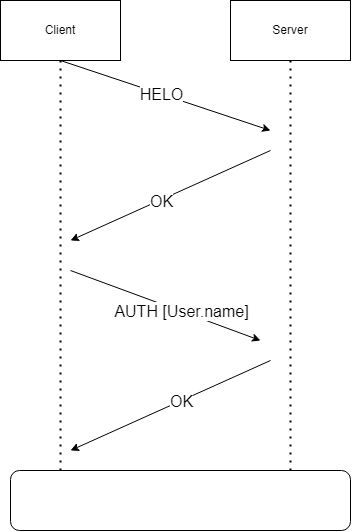
\includegraphics[scale=0.3]{Client-server 1.drawio.png}
\caption{Handshake Protocol WorkFlow}
\end{center}
\end{figure}


Jobs will be written as Server[Type][State][BootupTime][HourlyTime][Core][Memory][Disk]. An example of a Job format is: 37 0 653 3 700 3800. Through the GETS command, The client will use the "GETS ALL" or "GETS Capable [Job Format], enabling the server to send the amount of available jobs to the client. The client will reply with "OK" as an acknowledge that it has received the job lists from the server. This will continue until the server has sent a "." to depict that there are no more available information left to send to the client. The client will now begin the job scheduling using this command: SCHD[JobID]Server.Type][Server.ID], an example is SCHD 0 large 0. Once the job has been scheduled, the server will inform the client. Enabling for a loop until all the available jobs have been read and there are no more available.

\begin{figure}[H]
\begin{center}
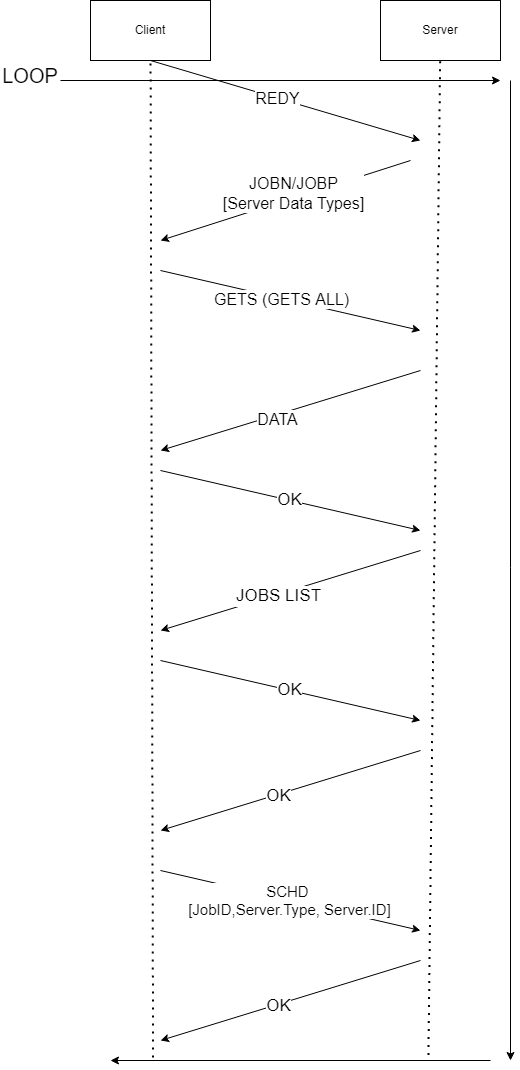
\includegraphics[scale=0.3]{Client-server LOOP.drawio.png}
\caption{Job Scheduling Loop Workflow}
\end{center}
\end{figure}

Once all the server files have been read and the "." has been detected. No more new data is required to be read by the Client. 

\begin{figure}[H]
\begin{center}
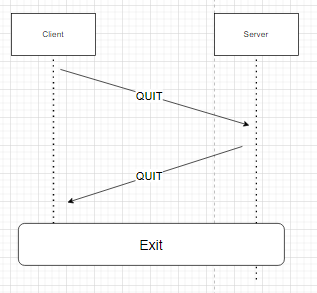
\includegraphics[scale=0.5]{Client-server QUIT.drawio.png}
\caption{Quit Command Workflow}
\end{center}
\end{figure}

\section{Design}
\label{sec:section3}
In this section, The client-side simulators and the functions that it uses to connect to the server-side simulator will be described, its use of the handshake protocol and the receiving and scheduling of jobs. This will be ordered accordingly in the client's order of operation.

\subsection{Connection and Communication with Server}
The client initally has an empty TCP socket (null), a TCP socket will be created and connected with an IP address of "localhost" and using port 50000. The purpose of the TCP Socket is to enable communication between the input and output streams of the server-side and client-side simulators. The BufferReader\cite{bufferreader} is used to read the data sent from the server with the DataOutputStream doing the contrary, its purpose being to send data by the Client. Lastly, to end the connection to the server if no data is left to be received by the client or server, a conditional statement "QUIT" be received. 

\subsection{Handshake Protocol}
The Client needs to perform a handshake protocol \cite{handshake} before it can connect to the Server. Firstly, the Client will initiate the handshake protocol through the "HELO" message, then converting this message into bytes. Once converted and sent to the Server, the Server will respond by sending in bytes that correlate to an "OK" message. 
\bigskip

A similar process will occur in the following step, The client will continue the handshake protocol by writing the "AUTH[User.name]" message for user authentication purposes, then converting the message to bytes. Once converted and sent, the Server will respond by sending an "OK message. 
\bigskip

The BufferReader and DataOutputStream are the two vital components used to make any request to the Server.

\subsection{Server Information and Receiving Jobs}
The BufferReader and DataOutputStream are used to receive jobs and server information. When the "REDY" and "GETS" Command are inputted by the client and sent to the server, once the server receives the bytes that correlate to these commands. The server will send the client's next available job as well as respective server information. This will be an incremental loop that loops and gathers through the server information, allowing for the BufferReader to read multiple lines that is send by the Server. DataOutputStream however is used to confirm that the data send from the server before the client can initiate the process of job scheduling.

\subsection{Job Scheduling }
The DataOutputStream will run the SCHD command as well with its respective extracted data elements. A sorting function is implemented to sort the Server with largest amount of cores first, ensuring the correct information is shared. After the jobs are scheduled, client the client will either continue to receive and schedule for the next job or exit the client simulator.

\section{Implementation}
\label{sec:section4}

\subsection{Software Libraries}
Software libraries are imported for various functions for the client side simulator. "java.net.*" was imported for the use of the sockets that would be used by the BufferReader and DataOutputStream.

\begin{figure}[H]
\begin{center}
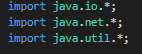
\includegraphics[scale=0.6]{Software Libraries.png}
\caption{Software Libraries}
\end{center}
\end{figure}

\subsection{Software}
Oracle VM VirtualBox running on the Linux Ubuntu Virtual Machine (VM) will be used for this project, for the purpose of depicting a distributing systems simulation (ds-sim). Visual Studio Code\cite{vsc} will be used within the VM to create, edit and debug the source code within the simulation. Ubuntu's terminal will be used to compile the client-side simulator, enabling tests to be ran with the server.

\subsection{Data Structures}
ArrayLists are used to store server data to be extracted for information. It will be extracted from the parser into a list, where it could be used later on if required.

\subsection{Implementation of Code}
\subsubsection{Software Libraries}
"Java.util.*" is used to import ArrayLists and Lists that stored the parsed Server Data. "Java.net.*" is used to create and store all the required classes and other relevant functions required. For further information, refer to Section 4.1.

\subsubsection{Connecting to Server}
An empty socket will be created initially. To connect to the server, it will initialise to "localhost" IP address and port 50000. For Client and Server to communicate with one another, BufferReader and DataOutputStream variables have been created to set and initialise with the socket.

\begin{figure}[H]
\begin{center}
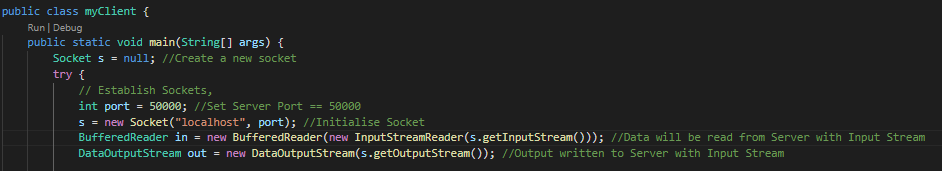
\includegraphics[scale=0.6]{Server Connection.png}
\caption{Server Connection Establishment}
\end{center}
\end{figure}

\subsubsection{HandShake Protocol}
The purpose of the "out.write(([Command\n].getBytes))" is to send and convert messages into bytes to the Server. "System.out.println()" is a java command used to print to the console what the server responds with. The "in.Readline();" purpose is to read that messages being received from the Server. It will initiate the Handshake with the "HELO" message.
\bigskip

With the authentication of usernames, a username will be stored as a String in the system and inputted during authentication. However, as this server does not currently possess any authentication processes as of now, anything inputted after the "AUTH" Command would display the same result.

\begin{figure}[H]
\begin{center}
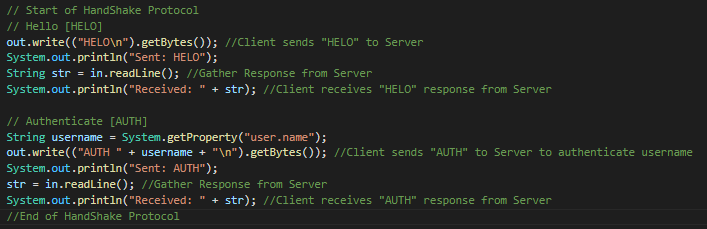
\includegraphics[scale=0.5]{HandShake Protocol.png}
\caption{HandShake Protocol}
\end{center}
\end{figure}

\subsubsection{ServerList}
Client will receive server data from Server, the received information will be converted and placed into a ServerList for later use. An "OK" message will be sent to the Server to indicate that Server Data has been received successfully. This process will continue until there is no more data available to check. Next, the servers will be sorted in ascending size where the largest server will be determined in the following step, for the purpose of job scheduling.

\begin{figure}[H]
\begin{center}
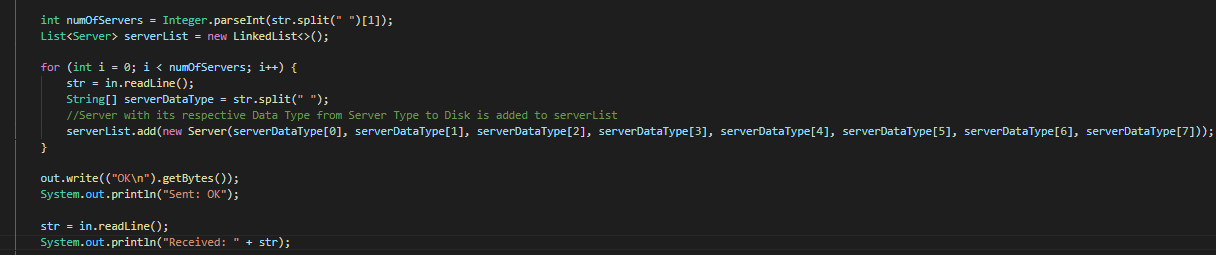
\includegraphics[scale=0.5]{ServerData.png}
\caption{ServerList}
\end{center}
\end{figure}

\subsubsection{Job Scheduler with Largest Round Robin (LRR)}
Job Scheduler will compare if Server Type equates to JOBN/JOBP, incrementing through the ServerList. The Detected Jobs will be converted from the Server as Bytes where it will be read in the 'JobSchedule' Format through the Terminal. This process will increment until a "." has been detected, indicating that there are no more available data to be read, causing the process to terminate.

\begin{figure}[H]
\begin{center}
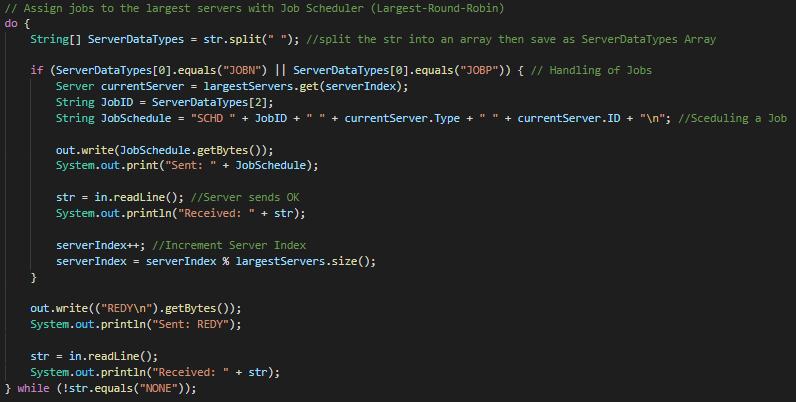
\includegraphics[scale=0.5]{LRR.png}
\caption{Largest Round Robin}
\end{center}
\end{figure}

\subsubsection{Server Class and Parser}
A server class will initialise different data types within the Server itself. Every Data Type will be different and unique within the Server class. The parse functions \cite{parse} will be used to convert any String functions to an integer, enabling them to be passed throughout the Client-side simulator.


\begin{figure}[H]
\begin{center}
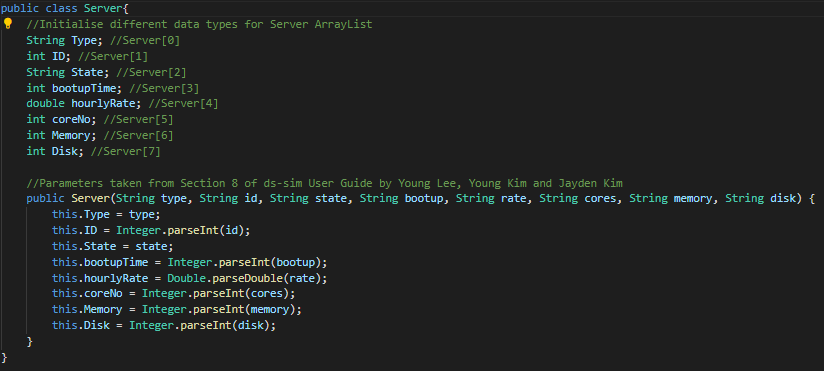
\includegraphics[scale=0.5]{Server.java.png}
\caption{Server Data Types}
\end{center}
\end{figure}


%----------------------------------------------------------------------------------------
%	REFERENCE LIST
%----------------------------------------------------------------------------------------

\bibliographystyle{ieeetr}
\bibliography{comp3100project}

\printbibliography

%----------------------------------------------------------------------------------------

\end{document}